\icode{E-MI-MU-L3-261113-001}
如图所示，质量均为 $m$ 的长方体物块 \(A\)、\(B\) 叠放在倾角为 $\theta$ 的固定斜面上，初始时在某约束下 \(A\)、\(B\) 均处于静止状态。已知 \(B\) 与斜面之间的动摩擦因数为 $\mu$，\(A\)、\(B\) 之间的动摩擦因数为 $\frac{1}{2}\mu$，且 $\mu = \tan \theta$，认为最大静摩擦力等于滑动摩擦力。若去除约束的同时，迅速给 \(A\) 或 \(B\) 一平行于斜面方向的力 $F$。下列情况能使 \(A\)、\(B\) 保持相对静止的是\paren[]

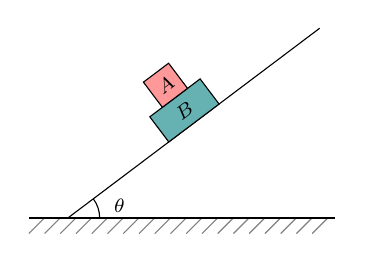
\begin{tikzpicture}[font=\scriptsize]
	\def\TheTa{37}%旋转角度
	\def\LenGth{4}%斜面
	\pgfmathsetmacro\CosLenGth{\LenGth*cos(\TheTa)}
	\begin{scope}[rotate=\TheTa]	
	    \draw (0,0)--++(\LenGth,0);
		\draw[fill=teal!60] (1.6,0) rectangle(2.4,.4)node[midway,rotate=\TheTa]{\(B\)};
		\draw[fill=red!40] (1.8,.4) rectangle(2.2,.8)node[midway,rotate=\TheTa]{\(A\)};
	\end{scope}
	\draw (.4,0) arc(0:\TheTa:.4);
	\node at(.65,.15){\(\theta\)};
	\foreach \x in{-.5,-.3,...,\CosLenGth}
		\draw[gray] (\x,-.2)--++(.2,.2);
	\draw[thick] (-.5,0)--({\CosLenGth+.2},0);
\end{tikzpicture}
\begin{choices}
	\item 若 $F$ 作用在 A 上，方向沿斜面向下，大小满足 $\frac{1}{2}mg\sin \theta \leq F \leq \frac{3}{2}mg\sin \theta$
	\item 若 $F$ 作用在 A 上，方向沿斜面向上，大小满足 $\frac{1}{2}mg\sin \theta \leq F \leq \frac{3}{2}mg\sin \theta$
	\item 若 $F$ 作用在 B 上，方向沿斜面向上，大小满足 $mg\sin \theta \leq F \leq 3mg\sin \theta$
	\item 若 $F$ 作用在 B 上，方向沿斜面向下，大小满足 $mg\sin \theta \leq F \leq 3mg\sin \theta$
\end{choices}
\begin{answer}
	BD\qquad 提示：
\end{answer}